We compare the performance of DPC \eqref{E:dpc} against an equivalent MPC formulation \eqref{E:mpc}. The solution obtained from MPC sets the benchmark that we compare to. Note that the MPC implementation uses the exact knowledge of the plant dynamics. Therefore, the associated control strategy is indeed the optimal strategy for the plant.

The performance is compared for 3 days in winter, i.e. January 28-31 and 3 days in summer, i.e. May 1-3. These are shown on the same plots in Figure~\ref{F:comparison}.
The sampling time in the simulations is 1 hr. The control horizon $N$ and the order of autoregression are both 6 hrs. The training procedure required a few minutes in the case of trees and 2 hrs for forests on a Win 10 machine with an i7 processor and 8GB memory.
The cooling usage factor $\mathsf{C}$ is constrained in $[0,1]$, the heat input in $[0,23]\ \mathrm{W/m^2}$, and the room temperature in $[19,25]\ \mathrm{^oC}$ during the winters and $[20,26]\ \mathrm{^oC}$ during the summers.
The optimization is solved using CPLEX \cite{IBM}.

The external disturbances - solar gain, internal gain due to equipment and dry-bulb temperature during the chosen periods are shown in Figure~\ref{F:dist}. The internal gain due to occupancy was proportional to the gain due to equipment. 
The reference temperature is chosen to be 22 $\mathrm{^oC}$. Due to cold weather, which is evident from the dry-bulb temperature, the heating system is switched on during the night to maintain the thermal comfort requirements. When the building is occupied during the day, due to excessive internal gain, the building requires cooling. The lighting in the building is adjusted to meet the minimum light requirements.
The optimal cooling usage factor and the radiator power for MPC, DPC-En and DPC-RT are shown in Figure~\ref{F:control1} and Figure~\ref{F:control2}, respectively. The control strategy with DPC-En shows a remarkable similarity to MPC, switching on/off the equipments at the same time with similar usage. However, the performance with DPC-RT is much different and worse. DPC-RT inherently suffers from high variance which is also evident in the control strategy, thus making it unsuitable for practical purposes. 
Although it seems like that adding the rate constraints to DPC-En would smoothen its behavior, this was avoided because the sampling time of the system is 1 hr which is already too high. The room temperature profile in Figure~\ref{F:state} is close to the reference in the case of DPC-En as well as MPC. 
Figure~\ref{F:obj} shows that the cumulative cost of the objective function is, as expected, minimum for MPC, and a bit higher for DPC-En. The cost for DPC-RT blows up around 12 noon on 30$^{th}$ January as one of the slack variables is non-zero, which happens due to high model inaccuracy.

The quantitative performance comparison is shown in Table~\ref{T:comparison}. MPC tracks the reference more closely at the expense of higher input costs in comparison to DPC-En. The higher cost of the inputs in MPC is also due to lighting. DPC-En explains 70.1\% variation in the optimal control strategies obtained from MPC while DPC-RT explains only 1.8\%. The mean optimal cost of DPC-En is more than MPC, and is maximum for DPC-RT due to a constraint violation.

\begin{table}[h!]
	\centering
	\begin{tabular}{ccccc}
		\toprule
		& explained & mean objective& mean input  & mean  \\
		&  variance$[\mathrm{-}]$ & value $[\mathrm{-}]$ & cost $[-]$ & deviance $[\mathrm{^oC}]$ \\     
		\midrule
		MPC    &  $\mathrm{-}$ &  22.60 & 17.16  &  0.26  \\
		DPC-En   & 70.1\% &  39.26  & 15.12 &  0.48 \\
		DPC-RT  & 1.8\% & 204.55 & 16.84 &  0.57 \\
		\bottomrule
	\end{tabular}
	\vspace{0.2cm}
	\caption{Quantitative comparison of explained variance, mean value of objective function, mean input cost $c^\top u$ and mean deviance from the reference temperature $|\mathsf{T}-\mathsf{T}_{\mathrm{ref}}|$.}
	\captionsetup{justification=centering}
	\label{T:comparison}
\end{table}

\begin{figure}[t!]
	\begin{center}
	\vspace{1.1cm}
	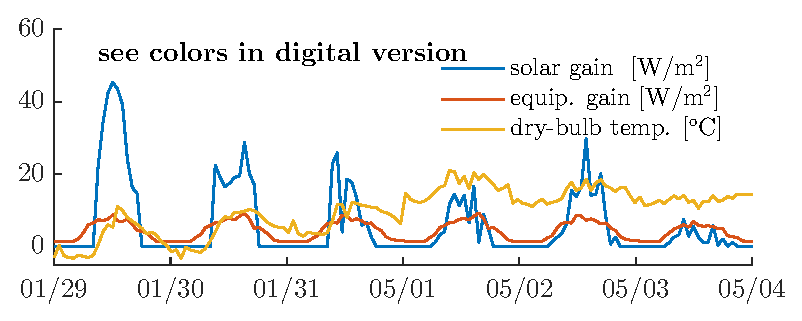
\includegraphics[width=23pc]{figures/disturbances.eps}
	\caption{External disturbances: solar gain, internal gain due to equipment and dry-bulb temperature.}
	\label{F:dist}
\end{center}
\end{figure}
\begin{figure}[h!]
\begin{center}
		\subfigure[Optimal cooling factor $\mathsf{C}$. DPC-En control strategy very similar to MPC.]{
		\label{F:control1}
		\centering
		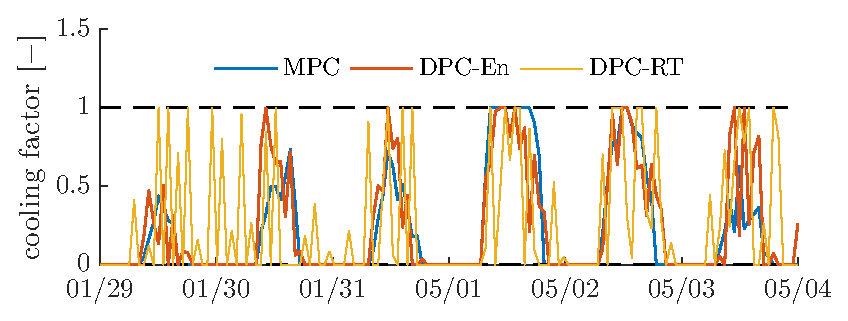
\includegraphics[width=23pc]{figures/input3.eps}
	}

	\subfigure[Optimal radiator heat $\mathsf{H}$. DPC-En control strategy very similar to MPC.]{
		\label{F:control2}
		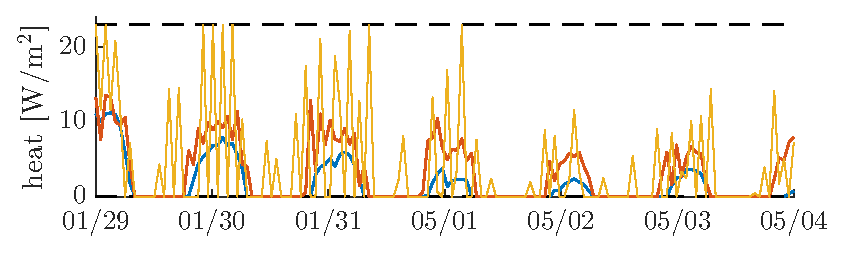
\includegraphics[width=23pc]{figures/input4.eps}
	}

	\subfigure[Room temp. has time varying bounds. When building is occupied, constraints are relaxed. MPC and DPC-En track the ref. temp. ($22 \ \mathrm{^oC}$) closely.]{
		\label{F:state}
		\centering
		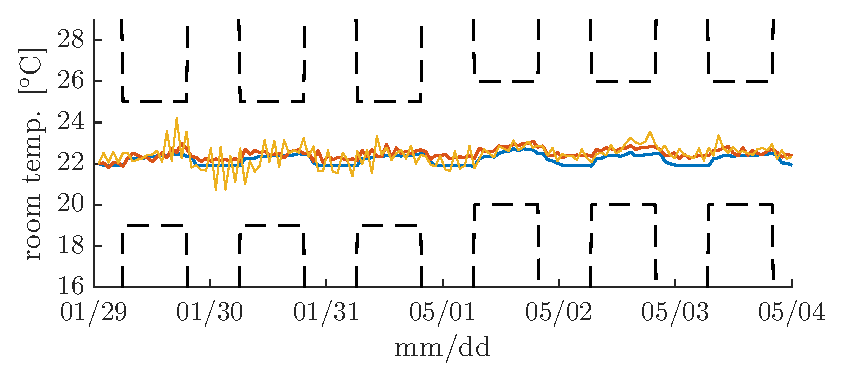
\includegraphics[width=23pc]{figures/state.eps}
	}

	\subfigure[Cumulative optimal cost after solving optimization. MPC serves as the benchmark with the minimum cost, followed by DPC-En and then DPC-RT.]{
		\label{F:obj}
		\centering
		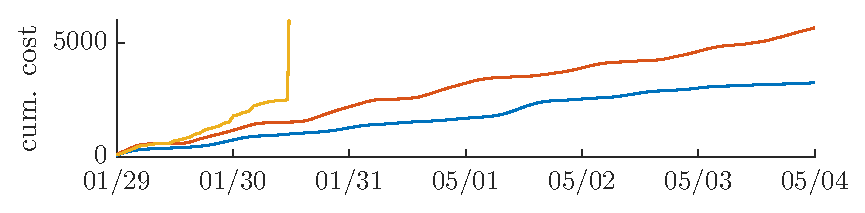
\includegraphics[width=23pc]{figures/cumsumcost.eps}
	}
	\end{center}
	\vspace{-0.6cm}
	\caption{Comparison of optimal performance obtained with MPC, DPC-En and DPC-RT for 3 days in January and 3 days in May.}
	\label{F:comparison}
	\captionsetup{justification=centering}
	\vspace{-0.3cm}
\end{figure}
Thus, we have shown that DPC-En provides a comparable performance to MPC without using the physical model.
However, one major limitation of the bilinear model is that the information about the building power consumption is not available. Much nonlinearities in the system are due to equipment efficiencies which are not considered in the bilinear case but are very important for practical purposes. 

Therefore, our next goal is to apply DPC-En on even more complex and realistic EnergyPlus model for which building a model predictive controller is time and cost prohibitive \cite{Sturzenegger2016}. This is because we would need to model intricate details like the geometry and construction layouts, the equipment design and layout plans, material properties, equipment and operational schedules etc.

